\documentclass{wissdoc}
% Autor: Roland Bless 1996-2009, bless <at> kit.edu
% ----------------------------------------------------------------
% Diplomarbeit - Hauptdokument
% ----------------------------------------------------------------
%%
%% $Id: thesis.tex 65 2012-05-10 10:32:11Z bless $
%%
% wissdoc Optionen: draft, relaxed, pdf --> siehe wissdoc.cls
% ------------------------------------------------------------------
% Weitere packages: (Dokumentation dazu durch "latex <package>.dtx")
\usepackage[numbers,sort&compress]{natbib}
% \usepackage{varioref}
% \usepackage{verbatim}
% \usepackage{float}    %z.B. \floatstyle{ruled}\restylefloat{figure}
% \usepackage{subfigure}
% \usepackage{fancybox} % für schattierte,ovale Boxen etc.
% \usepackage{tabularx} % automatische Spaltenbreite
% \usepackage{supertab} % mehrseitige Tabellen
% \usepackage[svnon,svnfoot]{svnver} % SVN Versionsinformation 
%% ---------------- end of usepackages -------------

%\svnversion{$Id: thesis.tex 65 2012-05-10 10:32:11Z bless $} % In case that you want to include version information in the footer

%% Informationen für die PDF-Datei
\hypersetup{
 pdfauthor={Chi Trung.Nguyen.},
 pdftitle={Not set}
 pdfsubject={Not set},
 pdfkeywords={Not set}
}

% Macros, nicht unbedingt notwendig
%%%%%%%%%%%%%%%%%%%%%%%%%%%%%%%%%%%%%%%%%%%%%%%%%%%%%%%%%%
% macros.tex -- einige mehr oder weniger nuetzliche Makros
% Autor: Roland Bless 1998
%%%%%%%%%%%%%%%%%%%%%%%%%%%%%%%%%%%%%%%%%%%%%%%%%%%%%%%%%%
% $Id: macros.tex 33 2007-01-23 09:00:59Z bless $
%%%%%%%%%%%%%%%%%%%%%%%%%%%%%%%%%%%%%%%%%%%%%%%%%%%%%%%%%%


%%%%%%%%%%%%%%%%%%%%%%%
% Kommentare 
%%%%%%%%%%%%%%%%%%%%%%%
\ifnotdraftelse{
\newcommand{\Kommentar}[1]{}
}{\newcommand{\Kommentar}[1]{{\em #1}}}
% Alles innerhalb von \Hide{} oder \ignore{} 
% wird von LaTeX komplett ignoriert (wie ein Kommentar)
\newcommand{\Hide}[1]{}
\let\ignore\Hide

%%%%%%%%%%%%%%%%%%%%%%%%%
% Leere Seite ohne Seitennummer, wird aber gezaehlt
%%%%%%%%%%%%%%%%%%%%%%%%%

\newcommand{\leereseite}{% Leerseite ohne Seitennummer, nächste Seite rechts (wenn 2-seitig)
 \clearpage{\pagestyle{empty}\cleardoublepage}
}
%%%%%%%%%%%%%%%%%%%%%%%%%%
% Flattersatz rechts und Silbentrennung, Leerraum nach rechts maximal 1cm
%%%%%%%%%%%%%%%%%%%%%%%%%%
\makeatletter
\newcommand{\myraggedright}{%
 \let\\\@centercr\@rightskip 0pt plus 1cm
 \rightskip\@rightskip
  \leftskip\z@skip
  \parindent\z@
  \spaceskip=.3333em
  \xspaceskip=.5em}
\makeatother

\makeatletter
\newcommand{\mynewline}{%
 \@centercr\@rightskip 0pt plus 1cm
}
\makeatother


%%%%%%%%%%%%%%%%%%%%%%%%%%
% Für Index
%%%%%%%%%%%%%%%%%%%%%%%%%%
\makeatletter
\def\mydotfill{\leavevmode\xleaders\hb@xt@ .44em{\hss.\hss}\hfill\kern\z@}
\makeatother
\def\bold#1{{\bfseries #1}}
\newbox\dbox \setbox\dbox=\hbox to .4em{\hss.\hss} % dot box for leaders
\newskip\rrskipb \rrskipb=.5em plus3em % ragged right space before break
\newskip\rrskipa \rrskipa=-.17em plus -3em minus.11em % ditto, after
\newskip\rlskipa \rlskipa=0pt plus3em % ragged left space after break
\newskip\rlskipb \rlskipb=.33em plus-3em minus.11em % ragged left before break
\newskip\lskip \lskip=3.3\wd\dbox plus1fil minus.3\wd\dbox % for leaders
\newskip \lskipa \lskipa=-2.67em plus -3em minus.11em %after leaders
\mathchardef\rlpen=1000 \mathchardef\leadpen=600
\def\rrspace{\nobreak\hskip\rrskipb\penalty0\hskip\rrskipa}
\def\rlspace{\penalty\rlpen\hskip\rlskipb\vadjust{}\nobreak\hskip\rlskipa}
\let\indexbreak\rlspace
\def\raggedurl{\penalty10000 \hskip.5em plus15em \penalty0 \hskip-.17em plus-15em minus.11em}
\def\raggeditems{\nobreak\hskip\rrskipb \penalty\leadpen \hskip\rrskipa %
\vadjust{}\nobreak\leaders\copy\dbox\hskip\lskip %
\kern3em \penalty\leadpen \hskip\lskipa %
\vadjust{}\nobreak\hskip\rlskipa}
\renewcommand*\see[2]{\rlspace\emph{\seename}~#1} % from makeidx.sty

%%%%%%%%%%%%%%%%%%%%%%%%%%
% Neue Seite rechts, leere linke Seite ohne Headings
%%%%%%%%%%%%%%%%%%%%%%%%%%
\newcommand{\xcleardoublepage}
{{\pagestyle{empty}\cleardoublepage}}

%%%%%%%%%%%%%%%%%%%%%%%%%%
% Tabellenspaltentypen (benoetigt colortbl)
%%%%%%%%%%%%%%%%%%%%%%%%%%
\newcommand{\PBS}[1]{\let\temp=\\#1\let\\=\temp}
\newcolumntype{y}{>{\PBS{\raggedright\hspace{0pt}}}p{1.35cm}}
\newcolumntype{z}{>{\PBS{\raggedright\hspace{0pt}}}p{2.5cm}}
\newcolumntype{q}{>{\PBS{\raggedright\hspace{0pt}}}p{6.5cm}}
\newcolumntype{g}{>{\columncolor[gray]{0.8}}c} % Grau
\newcolumntype{G}{>{\columncolor[gray]{0.9}}c} % helleres Grau

%%%%%%%%%%%%%%%%%%%%%%%%%%
% Anführungszeichen oben und unten
%%%%%%%%%%%%%%%%%%%%%%%%%%
\newcommand{\anf}[1]{"`{#1}"'}

%%%%%%%%%%%%%%%%%%%%%%%%%%
% Tiefstellen von Text
%%%%%%%%%%%%%%%%%%%%%%%%%%
% S\tl{0} setzt die 0 unter das S (ohne Mathemodus!)
% zum Hochstellen gibt es uebrigens \textsuperscript
\makeatletter
\DeclareRobustCommand*\textlowerscript[1]{%
  \@textlowerscript{\selectfont#1}}
\def\@textlowerscript#1{%
  {\m@th\ensuremath{_{\mbox{\fontsize\sf@size\z@#1}}}}}
\let\tl\textlowerscript
\let\ts\textsuperscript
\makeatother

%%%%%%%%%%%%%%%%%%%%%%%%%%
% Gauß-Klammern
%%%%%%%%%%%%%%%%%%%%%%%%%%
\newcommand{\ceil}[1]{\lceil{#1}\rceil}
\newcommand{\floor}[1]{\lfloor{#1}\rfloor}

%%%%%%%%%%%%%%%%%%%%%%%%%%
% Average Operator (analog zu min, max)
%%%%%%%%%%%%%%%%%%%%%%%%%%
\def\avg{\mathop{\mathgroup\symoperators avg}}

%%%%%%%%%%%%%%%%%%%%%%%%%%
% Wortabkürzungen
%%%%%%%%%%%%%%%%%%%%%%%%%%
\def\zB{z.\,B.\ }
\def\dh{d.\,h.\ }
\def\ua{u.\,a.\ }
\def\su{s.\,u.\ }
\newcommand{\bzw}{bzw.\ }

%%%%%%%%%%%%%%%%%%%%%%%%%%%%%%%%%%%
% Einbinden von Graphiken
%%%%%%%%%%%%%%%%%%%%%%%%%%%%%%%%%%%
% global scaling factor
\def\gsf{0.9}
%% Graphik, 
%% 3 Argumente: Datei, Label, Unterschrift
\newcommand{\Abbildung}[3]{%
\begin{figure}[tbh] %
\centerline{\scalebox{\gsf}{\includegraphics*{#1}}} %
\caption{#3} %
\label{#2} %
\end{figure} %
}
\let\Abb\Abbildung
%% Abbps
%% Graphik, skaliert, Angabe der Position
%% 5 Argumente: Position, Breite (0 bis 1.0), Datei, Label, Unterschrift
\newcommand{\Abbildungps}[5]{%
\begin{figure}[#1]%
\begin{center}
\scalebox{\gsf}{\includegraphics*[width=#2\textwidth]{#3}}%
\caption{#5}%
\label{#4}%
\end{center}
\end{figure}%
}
\let\Abbps\Abbildungps
%% Graphik, Angabe der Position, frei wählbares Argument für includegraphics
%% 5 Argumente: Position, Optionen, Datei, Label, Unterschrift
\newcommand{\Abbildungpf}[5]{%
\begin{figure}[#1]%
\begin{center}
\scalebox{\gsf}{\includegraphics*[#2]{#3}}%
\caption{#5}%
\label{#4}%
\end{center}
\end{figure}%
}
\let\Abbpf\Abbildungpf

%%
% Anmerkung: \resizebox{x}{y}{box} skaliert die box auf Breite x und Höhe y,
%            ist x oder y ein !, dann wird das usprüngliche 
%            Seitenverhältnis beibehalten.
%            \rescalebox funktioniert ähnlich, nur das dort ein Faktor
%            statt einer Dimension angegeben wird.
%%
% \Abbps{Position}{Breite in Bruchteilen der Textbreite}{Dateiname}{Label}{Bildunterschrift}
%

\newcommand{\refAbb}[1]{%
s.~Abbildung \ref{#1}}

%%%%%%%%%%%%%%%%%%%%
%% end of macros.tex
%%%%%%%%%%%%%%%%%%%%

% Print URLs not in Typewriter Font
\def\UrlFont{\rm}

\newcommand{\blankpage}{% Leerseite ohne Seitennummer, nächste Seite rechts
 \clearpage{\pagestyle{empty}\cleardoublepage}
}

%% Einstellungen für das gesamte Dokument

% Trennhilfen
% Wichtig! 
% Im ngerman-paket sind zusätzlich folgende Trennhinweise enthalten:
% "- = zusätzliche Trennstelle
% "| = Vermeidung von Ligaturen und mögliche Trennung (bsp: Schaf"|fell)
% "~ = Bindestrich an dem keine Trennung erlaubt ist (bsp: bergauf und "~ab)
% "= = Bindestrich bei dem Worte vor und dahinter getrennt werden dürfen
% "" = Trennstelle ohne Erzeugung eines Trennstrichs (bsp: und/""oder)

% Trennhinweise fuer Woerter hier beschreiben
\hyphenation{
% Pro-to-koll-in-stan-zen
% Ma-na-ge-ment  Netz-werk-ele-men-ten
% Netz-werk Netz-werk-re-ser-vie-rung
% Netz-werk-adap-ter Fein-ju-stier-ung
% Da-ten-strom-spe-zi-fi-ka-tion Pa-ket-rumpf
% Kon-troll-in-stanz
}

% Index-Datei öffnen
\ifnotdraft{\makeindex}
%%%%%%%%%%%%%% includeonly %%%%%%%%%%%%%%%%%%%
% Es werden nur die Teile eingebunden, die hier 
% aufgefuehrt sind!
\includeonly{%
titelseite,%
erklaerung,% Ist in KA Pflicht für Diplomarbeiten
einleitung,% Motivation, Zielsetzung, Gliederung
grundlagen,% Grundlagen 
analyse,   % Problembeschreibung (Detail) und Related Work
entwurf,   % Beschreibung der Problemlösung (Konzepte, allg. Architektur, ...)
implemen,  % Beschreibung der Umsetzung/Implementierung
eval,      % Nachweis und Auswertung
zusammenf  % Zusammenfassung der Ergebnisse und Ausblick
}
%%%%%%%%%%%%%%%%%%%%%%%%%%%%%%%%%%%%%%%%%%%%%%
\begin{document}

\frontmatter
\pagenumbering{roman}
\ifnotdraft{
 %% Titelseite
%% Vorlage $Id: titelseite.tex 61 2012-05-03 13:58:03Z bless $

\def\usesf{}
\let\usesf\sffamily % diese Zeile auskommentieren für normalen TeX Font

\newsavebox{\Erstgutachter}
\savebox{\Erstgutachter}{\usesf Prof.~Dr.~Jens Wagner}
\newsavebox{\Zweitgutachter}
\savebox{\Zweitgutachter}{\usesf Prof.~Dr.~?.~?????????}

\begin{titlepage}
\setlength{\unitlength}{1pt}
\begin{picture}(0,0)(85,770)

\includegraphics[width=\paperwidth]{logos/HFTL_Deckblatt}
\end{picture}

\thispagestyle{empty}

%\begin{titlepage}
%%\let\footnotesize\small \let\footnoterule\relax
\begin{center}
\hbox{}
\vfill
{\usesf
{\huge\bfseries Speicherkomponenten eines PC's\\
             \par}
\vskip 1.8cm
Studienarbeit\\
von\\[2mm]
\vskip 1cm

{\large\bfseries Chi Trung Nguyen\\}
\vskip 1.2cm
an der Hochschule für Telekommunikation Leipzig\\
in der Studienrichtung Wirtschaftsinformatik\\
%Universität Karlsruhe (TH)\\[2ex]
\vskip 3cm
\begin{tabular}{p{5.5cm}l}
Erstgutachter: & \usebox{\Erstgutachter} \\
\end{tabular}
\vskip 3cm
Bearbeitungszeit:\qquad 11.Juni~2012 -- 11.Juli~2012
}
\end{center}
\vfill
\end{titlepage}
%% Titelseite Ende


%%% Local Variables: 
%%% mode: latex
%%% TeX-master: "thesis"
%%% End: 

 \blankpage % Leerseite auf Titelrückseite
 %
 % Die folgende Erklärung ist für Diplomarbeiten Pflicht
 % (siehe Prüfungsordnung), für Studienarbeiten nicht notwendig
 \thispagestyle{empty}
\vspace*{42\baselineskip}
\hbox to \textwidth{\hrulefill}
\par
Ich erkläre hiermit, dass ich die vorliegende Arbeit selbständig verfasst und
keine anderen als die angegebenen Quellen und Hilfsmittel verwendet habe.

München, den 11. Juli 2012

%%%%%%%%%%%%%%%%%%%%%%%%%%%%%%%%%%%%%%%%%%%%%%%%%%%%%%%%%%%%%%%%%%%%%%%%
%% Hinweis:
%%
%% Diese Erklärung wird von der Prüfungsordnung für Diplomarbeiten 
%% verlangt und ist zu unterschreiben. Für Studienarbeiten ist diese
%% Erklärung nicht zwingend notwendig, schadet aber auch nicht.
%%%%%%%%%%%%%%%%%%%%%%%%%%%%%%%%%%%%%%%%%%%%%%%%%%%%%%%%%%%%%%%%%%%%%%%%
\clearpage







 \blankpage % Leerseite auf Erklärungsrückseite
}
%
%% *************** Hier geht's ab ****************
%% ++++++++++++++++++++++++++++++++++++++++++
%% Verzeichnisse
%% ++++++++++++++++++++++++++++++++++++++++++
\ifnotdraft{
{\parskip 0pt\tableofcontents} % toc bitte einzeilig
\blankpage
%\listoffigures
%\blankpage
%\listoftables
%\blankpage
}


%% ++++++++++++++++++++++++++++++++++++++++++
%% Hauptteil
%% ++++++++++++++++++++++++++++++++++++++++++
\graphicspath{{Bilder/}}

\mainmatter
\pagenumbering{arabic}
%% Einleitung.tex
%% $Id: einleitung.tex 61 2012-05-03 13:58:03Z bless $
%%

\chapter{Einleitung}
\label{ch:Einleitung}
%% ==============================

In der digitalen Gesellschaft und im Zeitalter des Internets wird es immer wichtiger immer mehr Daten so schnell wie möglich zu speichern.  \textit{Ein Speicher (v. lat.: spicarium Getreidespeicher, aus spica Ähre)[...] ist ein Ort oder eine Einrichtung zum Einlagern von materiellen oder} \textbf{\textit{immateriellen}} \textit{Objekten.} \cite{wiki:Speicher}
\newline
Ein Speichermedium dient also zur kurz- oder langfristigen \glqq \textit{Einlagerung}\grqq{} bzw. Erhaltung von immateriellen Objekten – oder anders ausgedr"uckt Informationen. 
Es stellt sich die Frage: Was sind Informationen? \newline
Im Laufe der Geschichte wurde der Informationsbegriff immer wieder neu definiert. Für die Informatik ist die Beschreibung nach Claude Elwood Shannon\footnote[1]{Claude Elwood Shannon: * 30. April 1916 in Petoskey, Michigan; \textdagger{} 24. Februar in Melford, Massachusetts gilt als Begr"uender der Informationstheorie} relevant. Demnach muss man ein Zeichen als kleinste Informationseinheit und dessen statistische H"aufigkeit in einem Code als Information sehen. 
\newline
Die Information darf nicht mit dem Bedeutungsgehalt verwechselt werden. Eine Information die wenig Sinn ergibt ist einer Information mit großem Sinngehalt gleichwertig. Wichtiger zu betrachten ist die Wahrscheinlichkeit des Auftretens eines Zeichens im vorgegebenen Code. Je geringer diese ist, desto h"oher ist sein Informationsgehalt.
\\
Im wesentlichen werden Informationen auf Speichermedien aber in Form von Daten abgelegt. 
\\Mehrere aufeinanderfolgende Zeichen werden als Zeichenfolge bezeichnet.\cite{hansen:wi1}
\\ 
Daten sind nach ISO 2382 
\glqq \textit{Gebilde aus Zeichen oder kontinuierliche Funktionen, die aufgrund bekannter oder unterstellter Abmachungen Informationen darstellen, vorrangig zum Zweck der Verarbeitung und als deren Ergebnis.}\grqq{} 
\\
Somit sind nach einer bestimmten Syntax angeordneten Zeichen \textbf{Daten}.

%% ==============================
\section{Zielsetzung der Arbeit}
%% ==============================
\label{ch:Einleitung:sec:Zielsetzung}

Mit dieser Arbeit möchte ich auf grundlegende Prinzipien der Speicherung von Informationen auf verschiedenen Medien, insbesondere in der Informatik eingehen. Sie soll eine "Ubersicht auf M"oglichkeiten der Datenspeicherung im fr"uhen und heutigen Informationsalter schaffen und die Funktionsweise der Speichermedien erkl"aren. Auch wenn der Titel \glqq Speicherkomponenten eines PC \grqq{} ist, wird der Vollst"andigkeit halber trotzdem auf "altere, heute nicht mehr gebr"aubliche Wege Daten zu speichern R"ucksicht genommen. Der Leser sollte nach dem Lesen der Arbeit einen "Uberblick dar"uber haben, welche Methoden es gibt Informationen aufzubewahren. Es werden keine neuen wissenschaftlichen Erkenntnisse vorgestellt, sondern fachliche Informationen zusammengestellt.

%% ==============================
\section{Gliederung der Arbeit}
%% ==============================
\label{ch:Einleitung:sec:Gliederung}

Man unterscheidet zwischen technischer und nichttechnischer Speicherung. Die Speicherung von Informationen ist aber nicht einer Erfindung der Neuzeit. Seit jeher versucht der Mensch Informationen zu bewahren, damit diese nicht in Vergessenheit geraten. 
\\
So geh"oren auch H"ohlenmalereien dazu. Man sch"atzt, dass die "alteste H"ohlenmalerei etwa 40.000 Jahre alt ist. Bei dieser sogenannten nichttechnischen Speicherung ben"otigt es ein Tr"agermaterial wie Papier, Pergament, Papyrusrollen oder wie in diesem Beispiel Stein um Informationen zu erhalten. Ein gro"ser Nachteil kann jedoch die sp"atere Entzifferung der \glqq Daten\grqq{} sein, aber immerhin kann man diese sofort auslesen.
\\
Bei der technischen Speicherung bedarf es einer speziellen Methode um die gew"unschten Daten auszulesen. Diese sind nicht sofort per Auge oder mit der Hand erkennbar(vgl. Braille\footnote[2]{Braille: Schrift der Blinden. Die Schrift(verschiedene angeordnete Punkte) wird von Hinten auf Papier gepresst. Diese sind so mit den Fingern ertastbar}). 
%TODO: eingehen auf untere Kapitel(elektronische,magnetische speicherung etc
\\
Die Arbeit ist dementsprechend in diese beiden Teile strukturiert, wobei auf den nichttechnischen Teil nur kurz der Vollst"andigkeit halber eingegangen wird. 
\\
Zum Schluss wird versucht einen kleinen Ausblick auf die Entwicklung der Speicherkomponenten eines PC's zu geben.

%%% Local Variables: 
%%% mode: latex
%%% TeX-master: "thesis"
%%% End: 
  % Einleitung
%% grundlagen.tex
%% $Id: grundlagen.tex 61 2012-05-03 13:58:03Z bless $
%%

\chapter{Grundlagen}
\label{ch:Grundlagen}
%% ==============================
Die Grundlagen müssen soweit beschrieben
werden, dass ein Leser das Problem und
die Problemlösung  versteht.Um nicht zuviel 
zu beschreiben, kann man das auch erst gegen 
Ende der Arbeit schreiben.

Bla fasel\ldots

%% ==============================
\section{Abschnitt 1}
%% ==============================
\label{ch:Grundlagen:sec:Abschnitt1}

Bla fasel\ldots

%% ==============================
\section{Abschnitt 2}
%% ==============================
\label{ch:Grundlagen:sec:Abschnitt2}

Bla fasel\ldots

%% ==============================
\section{Verwandte Arbeiten}
%% ==============================
\label{ch:Grundlagen:sec:RelatedWork}
Hier kommt "`Related Work"' rein.
Eine Literaturrecherche sollte so vollständig wie möglich sein,
relevante Ansätze müssen beschrieben werden und es sollte deutlich 
gemacht werden, wo diese Ansätze Defizite aufweisen oder nicht
anwendbar sind, z.\,B. weil sie von anderen Umgebungen oder 
Voraussetzungen ausgehen.


Bla fasel\ldots

%%% Local Variables: 
%%% mode: latex
%%% TeX-master: "thesis"
%%% End: 
  % Grundlagen
%% analyse.tex
%% $Id: analyse.tex 61 2012-05-03 13:58:03Z bless $

\chapter{Analyse}
\label{ch:Analyse}
%% ==============================
In diesem Kapitel sollten zun�chst das zu l�sende Problem
sowie die Anforderungen und die Randbedingungen 
einer L�sung\index{L�sung} beschrieben werden (also nochmal
eine pr�zisierte Aufgabenstellung\index{Aufgabenstellung}).

Dann folgt �blicherweise ein �berblick �ber bereits existierende
L�sungen bzw. Ans�tze, die meistens andere Voraussetzungen bzw.
Randbedingungen annehmen.

Bla fasel\ldots

%% ==============================
\section{Anforderungen}
%% ==============================
\label{ch:Analyse:sec:Anforderungen}
Anforderungen und Randbedingungen\index{Randbedingungen} \ldots

%% ==============================
\section{Existierende L�sungsans�tze}
%% ==============================
\label{ch:Analyse:sec:RelatedWork}

Hier kommt eine ausf�hrliche Diskussion
von "`Related Work"'.

Bla fasel\ldots

%% ==============================
\section{Weiterer Abschnitt}
%% ==============================
\label{ch:Analyse:sec:Abschnitt}

Bla fasel\ldots hat auch schon \cite{TB2000} gesagt und
\cite{TB98,JSAC96,qosr} sollte man mal gelesen haben.
Abbildung~\ref{fig:test} auf S.~\pageref{fig:test} sollte man
sich mal anschauen.

Blindtext Blindtext Blindtext Blindtext Blindtext Blindtext Blindtext
Blindtext Blindtext Blindtext Blindtext Blindtext Blindtext Blindtext
Blindtext Blindtext Blindtext Blindtext Blindtext Blindtext Blindtext
Blindtext Blindtext Blindtext Blindtext Blindtext Blindtext Blindtext
Blindtext Blindtext Blindtext Blindtext Blindtext Blindtext Blindtext
Blindtext Blindtext Blindtext Blindtext Blindtext Blindtext Blindtext
Blindtext Blindtext Blindtext Blindtext Blindtext Blindtext Blindtext
Blindtext Blindtext Blindtext Blindtext Blindtext Blindtext Blindtext
Blindtext Blindtext Blindtext Blindtext Blindtext Blindtext Blindtext

Blindtext Blindtext Blindtext Blindtext Blindtext Blindtext Blindtext
Blindtext Blindtext Blindtext Blindtext Blindtext Blindtext Blindtext
Blindtext Blindtext Blindtext Blindtext Blindtext Blindtext Blindtext
Blindtext Blindtext Blindtext Blindtext Blindtext Blindtext Blindtext
Blindtext Blindtext Blindtext Blindtext Blindtext Blindtext Blindtext
Blindtext Blindtext Blindtext Blindtext Blindtext Blindtext Blindtext
Blindtext Blindtext Blindtext Blindtext Blindtext Blindtext Blindtext
Blindtext Blindtext Blindtext Blindtext Blindtext Blindtext Blindtext
Blindtext Blindtext Blindtext Blindtext Blindtext Blindtext Blindtext
Blindtext Blindtext Blindtext Blindtext Blindtext Blindtext Blindtext
Blindtext Blindtext Blindtext Blindtext Blindtext Blindtext Blindtext
Blindtext Blindtext Blindtext Blindtext Blindtext Blindtext Blindtext
Blindtext Blindtext Blindtext Blindtext Blindtext Blindtext Blindtext

Blindtext Blindtext Blindtext Blindtext Blindtext Blindtext Blindtext
Blindtext Blindtext Blindtext Blindtext Blindtext Blindtext Blindtext
Blindtext Blindtext Blindtext Blindtext Blindtext Blindtext Blindtext
Blindtext Blindtext Blindtext Blindtext Blindtext Blindtext Blindtext
Blindtext Blindtext Blindtext Blindtext Blindtext Blindtext Blindtext
Blindtext Blindtext Blindtext Blindtext Blindtext Blindtext Blindtext
Blindtext Blindtext Blindtext Blindtext Blindtext Blindtext Blindtext
Blindtext Blindtext Blindtext Blindtext Blindtext Blindtext Blindtext
Blindtext Blindtext Blindtext Blindtext Blindtext Blindtext Blindtext
Blindtext Blindtext Blindtext Blindtext Blindtext Blindtext Blindtext

Blindtext Blindtext Blindtext Blindtext Blindtext Blindtext Blindtext
Blindtext Blindtext Blindtext Blindtext Blindtext Blindtext Blindtext
Blindtext Blindtext Blindtext Blindtext Blindtext Blindtext Blindtext
Blindtext Blindtext Blindtext Blindtext Blindtext Blindtext Blindtext
Blindtext Blindtext Blindtext Blindtext Blindtext Blindtext Blindtext
Blindtext Blindtext Blindtext Blindtext Blindtext Blindtext Blindtext
Blindtext Blindtext Blindtext Blindtext Blindtext Blindtext Blindtext
Blindtext Blindtext Blindtext\index{Blindtext} Blindtext Blindtext Blindtext Blindtext

\begin{figure}[!htbp]
  \centering
  \fbox{\parbox{0.8\textwidth}{
  Abbildungen sollten m�glichst als EPS (Encapsulated Postscript) 
  bzw. PDF eingebunden werden.
  Zur Erzeugung sauberer EPS-Dateien empfiehlt sich das Tool \texttt{ps2eps}
  zur Nachbearbeitung von Postscript-Dateien. Mit \texttt{epstopdf} kann
  dann eine PDF-Datei zum Einbinden erzeugt werden.}}
  \caption{Testabbildung}
  \label{fig:test}
\end{figure}

Blindtext Blindtext Blindtext Blindtext Blindtext Blindtext Blindtext
Blindtext Blindtext Blindtext Blindtext Blindtext Blindtext Blindtext
Blindtext Blindtext Blindtext Blindtext Blindtext Blindtext Blindtext
Blindtext Blindtext Blindtext Blindtext Blindtext Blindtext Blindtext
Blindtext Blindtext Blindtext Blindtext Blindtext Blindtext Blindtext
Blindtext Blindtext Blindtext Blindtext Blindtext Blindtext Blindtext
Blindtext Blindtext Blindtext Blindtext Blindtext Blindtext Blindtext

Blindtext Blindtext Blindtext Blindtext Blindtext Blindtext Blindtext
Blindtext Blindtext Blindtext Blindtext Blindtext Blindtext Blindtext
Blindtext Blindtext Blindtext Blindtext Blindtext Blindtext Blindtext

Blindtext Blindtext Blindtext Blindtext Blindtext Blindtext Blindtext
Blindtext Blindtext Blindtext Blindtext Blindtext Blindtext Blindtext
Blindtext Blindtext Blindtext Blindtext Blindtext Blindtext Blindtext
Blindtext Blindtext Blindtext Blindtext Blindtext Blindtext Blindtext
Blindtext Blindtext Blindtext Blindtext Blindtext Blindtext Blindtext
Blindtext Blindtext Blindtext Blindtext Blindtext Blindtext Blindtext

Blindtext Blindtext Blindtext Blindtext Blindtext Blindtext Blindtext
Blindtext Blindtext Blindtext Blindtext Blindtext Blindtext Blindtext
Blindtext Blindtext Blindtext Blindtext Blindtext Blindtext Blindtext
Blindtext Blindtext Blindtext Blindtext Blindtext Blindtext Blindtext
Blindtext Blindtext Blindtext Blindtext Blindtext Blindtext Blindtext
Blindtext Blindtext Blindtext Blindtext Blindtext Blindtext Blindtext
Blindtext Blindtext Blindtext Blindtext Blindtext Blindtext Blindtext
Blindtext Blindtext Blindtext Blindtext Blindtext Blindtext Blindtext
Blindtext Blindtext Blindtext Blindtext Blindtext Blindtext Blindtext
Blindtext Blindtext Blindtext Blindtext Blindtext Blindtext Blindtext
Blindtext Blindtext Blindtext Blindtext Blindtext Blindtext Blindtext
Blindtext Blindtext Blindtext Blindtext Blindtext Blindtext Blindtext
Blindtext Blindtext Blindtext Blindtext Blindtext Blindtext Blindtext
Blindtext Blindtext Blindtext Blindtext Blindtext Blindtext Blindtext

Blindtext Blindtext Blindtext Blindtext Blindtext Blindtext Blindtext
Blindtext Blindtext Blindtext Blindtext Blindtext Blindtext Blindtext
Blindtext Blindtext Blindtext Blindtext Blindtext Blindtext Blindtext
Blindtext Blindtext Blindtext Blindtext Blindtext Blindtext Blindtext
Blindtext Blindtext Blindtext Blindtext Blindtext Blindtext Blindtext
Blindtext Blindtext Blindtext Blindtext Blindtext Blindtext Blindtext
Blindtext Blindtext Blindtext Blindtext Blindtext Blindtext Blindtext
Blindtext Blindtext Blindtext Blindtext Blindtext Blindtext Blindtext
Blindtext Blindtext Blindtext Blindtext Blindtext Blindtext Blindtext
Blindtext Blindtext Blindtext Blindtext Blindtext Blindtext Blindtext
Blindtext Blindtext Blindtext Blindtext Blindtext Blindtext Blindtext
%% ==============================
\section{Zusammenfassung}
%% ==============================
\label{ch:Analyse:sec:zusammenfassung}

Am Ende sollten ggf. die wichtigsten Ergebnisse nochmal in \emph{einem}
kurzen Absatz zusammengefasst werden.

%%% Local Variables: 
%%% mode: latex
%%% TeX-master: "thesis"
%%% End: 
     % Analyse
%% entwurf.tex
%% $Id: entwurf.tex 61 2012-05-03 13:58:03Z bless $
%%

\chapter{Entwurf}
\label{ch:Entwurf}
%% ==============================
In diesem Kapitel erfolgt die ausf�hrliche Beschreibung des eigenen
L�sungsansatzes. Dabei sollten L�sungsalternativen diskutiert und
Entwurfsentscheidungen dargelegt werden.


Bla fasel\ldots

%% ==============================
\section{Abschnitt 1}
%% ==============================
\label{ch:Entwurf:sec:Abschnitt1}

Bla fasel\ldots

%% ==============================
\section{Abschnitt 2}
%% ==============================
\label{ch:Entwurf:sec:Abschnitt2}

Bla fasel\ldots

Blindtext Blindtext Blindtext Blindtext Blindtext Blindtext Blindtext
Blindtext Blindtext Blindtext Blindtext Blindtext Blindtext Blindtext
Blindtext Blindtext Blindtext Blindtext Blindtext Blindtext Blindtext
Blindtext Blindtext Blindtext Blindtext Blindtext Blindtext Blindtext
Blindtext Blindtext Blindtext Blindtext Blindtext Blindtext Blindtext
Blindtext Blindtext Blindtext Blindtext Blindtext Blindtext Blindtext
Blindtext Blindtext Blindtext Blindtext Blindtext Blindtext Blindtext
Blindtext Blindtext Blindtext Blindtext Blindtext Blindtext Blindtext
Blindtext Blindtext Blindtext Blindtext Blindtext Blindtext Blindtext
Blindtext Blindtext Blindtext Blindtext Blindtext Blindtext Blindtext
Blindtext Blindtext Blindtext Blindtext Blindtext Blindtext Blindtext
Blindtext Blindtext Blindtext Blindtext Blindtext Blindtext Blindtext
Blindtext Blindtext Blindtext Blindtext Blindtext Blindtext Blindtext
Blindtext Blindtext Blindtext Blindtext Blindtext Blindtext Blindtext
Blindtext Blindtext Blindtext Blindtext Blindtext Blindtext Blindtext
Blindtext Blindtext Blindtext Blindtext Blindtext Blindtext Blindtext
Blindtext Blindtext Blindtext Blindtext Blindtext Blindtext Blindtext

Blindtext Blindtext Blindtext Blindtext Blindtext Blindtext Blindtext
Blindtext Blindtext Blindtext Blindtext Blindtext Blindtext Blindtext
Blindtext Blindtext Blindtext Blindtext Blindtext Blindtext Blindtext
Blindtext Blindtext Blindtext Blindtext Blindtext Blindtext Blindtext
Blindtext Blindtext Blindtext Blindtext Blindtext Blindtext Blindtext
Blindtext Blindtext Blindtext Blindtext Blindtext Blindtext Blindtext
Blindtext Blindtext Blindtext Blindtext Blindtext Blindtext Blindtext
Blindtext Blindtext Blindtext Blindtext Blindtext Blindtext Blindtext
Blindtext Blindtext Blindtext Blindtext Blindtext Blindtext Blindtext
Blindtext Blindtext Blindtext Blindtext Blindtext Blindtext Blindtext
Blindtext Blindtext Blindtext Blindtext Blindtext Blindtext Blindtext
Blindtext Blindtext Blindtext Blindtext Blindtext Blindtext Blindtext
Blindtext Blindtext Blindtext Blindtext Blindtext Blindtext Blindtext
Blindtext Blindtext Blindtext Blindtext Blindtext Blindtext Blindtext
Blindtext Blindtext Blindtext Blindtext Blindtext Blindtext Blindtext
Blindtext Blindtext Blindtext Blindtext Blindtext Blindtext Blindtext
Blindtext Blindtext Blindtext Blindtext Blindtext Blindtext Blindtext
Blindtext Blindtext Blindtext Blindtext Blindtext Blindtext Blindtext
Blindtext Blindtext Blindtext Blindtext Blindtext Blindtext Blindtext
Blindtext Blindtext Blindtext Blindtext Blindtext Blindtext Blindtext

Blindtext Blindtext Blindtext Blindtext Blindtext Blindtext Blindtext
Blindtext Blindtext Blindtext Blindtext Blindtext Blindtext Blindtext
Blindtext Blindtext Blindtext Blindtext Blindtext Blindtext Blindtext
Blindtext Blindtext Blindtext Blindtext Blindtext Blindtext Blindtext
Blindtext Blindtext Blindtext Blindtext Blindtext Blindtext Blindtext
Blindtext Blindtext Blindtext Blindtext Blindtext Blindtext Blindtext
Blindtext Blindtext Blindtext Blindtext Blindtext Blindtext Blindtext
Blindtext Blindtext Blindtext Blindtext Blindtext Blindtext Blindtext
Blindtext Blindtext Blindtext Blindtext Blindtext Blindtext Blindtext
Blindtext Blindtext Blindtext Blindtext Blindtext Blindtext Blindtext
Blindtext Blindtext Blindtext Blindtext Blindtext Blindtext Blindtext
Blindtext Blindtext Blindtext Blindtext Blindtext Blindtext Blindtext
Blindtext Blindtext Blindtext Blindtext Blindtext Blindtext Blindtext
Blindtext Blindtext Blindtext Blindtext Blindtext Blindtext Blindtext
Blindtext Blindtext Blindtext Blindtext Blindtext Blindtext Blindtext

Blindtext Blindtext Blindtext Blindtext Blindtext Blindtext Blindtext
Blindtext Blindtext Blindtext Blindtext Blindtext Blindtext Blindtext
Blindtext Blindtext Blindtext Blindtext Blindtext Blindtext Blindtext
Blindtext Blindtext Blindtext Blindtext Blindtext Blindtext Blindtext
Blindtext Blindtext Blindtext Blindtext Blindtext Blindtext Blindtext
Blindtext Blindtext Blindtext Blindtext Blindtext Blindtext Blindtext
Blindtext Blindtext Blindtext Blindtext Blindtext Blindtext Blindtext
Blindtext Blindtext Blindtext Blindtext Blindtext Blindtext Blindtext
Blindtext Blindtext Blindtext Blindtext Blindtext Blindtext Blindtext
Blindtext Blindtext Blindtext Blindtext Blindtext Blindtext Blindtext
Blindtext Blindtext Blindtext Blindtext Blindtext Blindtext Blindtext
Blindtext Blindtext Blindtext Blindtext Blindtext Blindtext Blindtext
Blindtext Blindtext Blindtext Blindtext Blindtext Blindtext Blindtext
Blindtext Blindtext Blindtext Blindtext Blindtext Blindtext Blindtext
Blindtext Blindtext Blindtext Blindtext Blindtext Blindtext Blindtext
Blindtext Blindtext Blindtext Blindtext Blindtext Blindtext Blindtext

Blindtext Blindtext Blindtext Blindtext Blindtext Blindtext Blindtext
Blindtext Blindtext Blindtext Blindtext Blindtext Blindtext Blindtext
Blindtext Blindtext Blindtext Blindtext Blindtext Blindtext Blindtext
Blindtext Blindtext Blindtext Blindtext Blindtext Blindtext Blindtext
Blindtext Blindtext Blindtext Blindtext Blindtext Blindtext Blindtext
Blindtext Blindtext Blindtext Blindtext Blindtext Blindtext Blindtext
Blindtext Blindtext Blindtext Blindtext Blindtext Blindtext Blindtext
Blindtext Blindtext Blindtext Blindtext Blindtext Blindtext Blindtext
Blindtext Blindtext Blindtext Blindtext Blindtext Blindtext Blindtext
Blindtext Blindtext Blindtext Blindtext Blindtext Blindtext Blindtext
Blindtext Blindtext Blindtext Blindtext Blindtext Blindtext Blindtext
Blindtext Blindtext Blindtext Blindtext Blindtext Blindtext Blindtext
Blindtext Blindtext Blindtext Blindtext Blindtext Blindtext Blindtext

%% ==============================
\section{Zusammenfassung}
%% ==============================
\label{ch:Entwurf:sec:zusammenfassung}

Am Ende sollten ggf. die wichtigsten Ergebnisse nochmal in \emph{einem}
kurzen Absatz zusammengefasst werden.

%%% Local Variables: 
%%% mode: latex
%%% TeX-master: "thesis"
%%% End: 
     % Entwurf
%% implemen.tex
%% $Id: implemen.tex 61 2012-05-03 13:58:03Z bless $
%%
% !TEX root = thesis.tex

\chapter{Implementierung}
\label{ch:Implementierung}
%% ==============================
Bla fasel\ldots

%% ==============================
\section{Abschnitt 1}
%% ==============================
\label{ch:Implementierung:sec:Abschnitt1}

Bla fasel\ldots

%% ==============================
\section{Abschnitt 2}
%% ==============================
\label{ch:Implementierung:sec:Abschnitt2}

Bla fasel\ldots

%%% Local Variables: 
%%% mode: latex
%%% TeX-master: "thesis"
%%% End: 
    % Implementierung
%% eval.tex
%% $Id: eval.tex 61 2012-05-03 13:58:03Z bless $
% !TEX root = thesis.tex

\chapter{Evaluierung}
\label{ch:Evaluierung}
%% ==============================
Hier kommt der Nachweis, dass das in Kapitel~\ref{ch:Entwurf}
entworfene Konzept auch funktioniert. Leistungsmessungen einer
Implementierung werden auch immer gerne gesehen.

Bla fasel\ldots

%% ==============================
\section{Abschnitt 1}
%% ==============================
\label{ch:Evaluierung:sec:Abschnitt1}

Bla fasel\ldots

%% ==============================
\section{Abschnitt 2}
%% ==============================
\label{ch:Evaluierung:sec:Abschnitt2}

Bla fasel\ldots

%% ==============================
\section{Zusammenfassung}
%% ==============================
\label{ch:Evaluierung:sec:zusammenfassung}

Am Ende sollten ggf. die wichtigsten Ergebnisse nochmal in \emph{einem}
kurzen Absatz zusammengefasst werden.

%%% Local Variables: 
%%% mode: latex
%%% TeX-master: "thesis"
%%% End: 
        % Evaluierung
%% zusammenf.tex
%% $Id: zusammenf.tex 61 2012-05-03 13:58:03Z bless $
%%

\chapter{Zusammenfassung und Ausblick}
\label{ch:Zusammenfassung}
%% ==============================
Zusammenfassend l"asst sich also sagen, dass es viele M"oglichkeiten heute gibt, Daten zu speichern. Die einen sind praktischer, die anderen etwas unpraktischer.
Der meist genutzte Massenspeicher ist im Moment wohl die Festplatte, seine Entwicklung war rasant – "ahnlich dem \textit{Mooreschen Gesetz} zeigt sie einen ann"ahernd exponentiellen Verlauf wie die Abbildung \ref{fig:kapazit} zeigt. Alle 16 Monate etwa, verdoppelt sich damit die Speicherkapazit"at
\begin{figure}[ht]
				\centering
				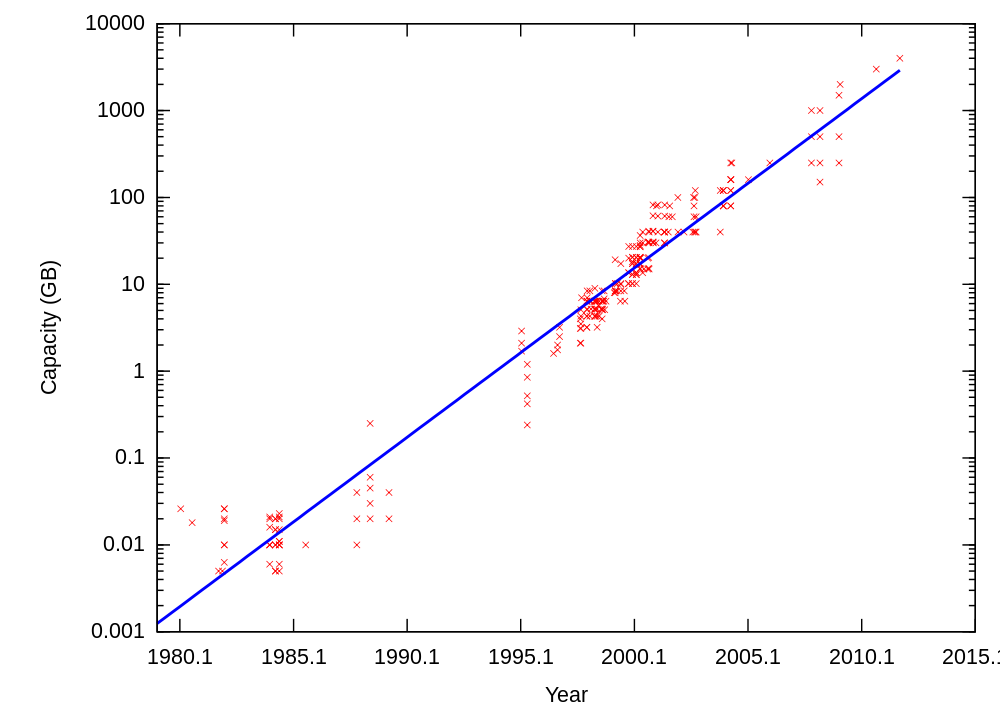
\includegraphics[width=0.7\textwidth]{images/kapazit} 
				\caption[Entwicklung Speicherkapazit"at Fesplatte in halblogarithmischer Skalierung \cite{fig:kapazit}]{Entwicklung Speicherkapazit"at Fesplatte in halblogarithmischer Skalierung}
				\label{fig:kapazit}
				\end{figure}
\\
Auch die Rohstoffverknappung k"onnte den Speicherhunger behindern, wie die Flutkatastrophe Ende 2011 in Thailand zeigte. Die Preise f"ur Festplatten stiegen darauf hin, da nahezu alle Festplatten der Marktriesen dort produziert wurden.
\\
Doch irgendwann wird die physikalische Grenze erreicht werden.
\\
Das Ziel ist 1 Bit = 1 Atom, das Speichern auf atomarer Ebene. Im Januar 2012 konnten die Forscher des IBM Almaden Research Centers zusammen mit Forschern der Max-Planck-Gesellschaft den kleinsten Speicher der Welt bauen. Sie haben es geschafft einen 12 Atom Speicher zu bauen, allerdings ist dieser nur bei -268 Grad zuverl"assig. Bis er bei Raumtemperaturen funktioniert und Marktreif ist, wird es wohl noch einige Zeit dauern.\cite{heise:ibm} 
\\
Dann wird es aber wohl m"oglich sein die gesamte Weltliteratur auf einen Speicher von der Gr"o"se einer Briefmarke zu speichern. 

%%% Local Variables: 
%%% mode: latex
%%% TeX-master: "thesis"
%%% End: 
   % Zusammenfassung und Ausblick

%% ++++++++++++++++++++++++++++++++++++++++++
%% Anhang
%% ++++++++++++++++++++++++++++++++++++++++++

\appendix
%\include{anhang_a}
%\include{anhang_b}

%% ++++++++++++++++++++++++++++++++++++++++++
%% Literatur
%% ++++++++++++++++++++++++++++++++++++++++++
%  mit dem Befehl \nocite werden auch nicht 
%  zitierte Referenzen abgedruckt
\cleardoublepage
\phantomsection
\addcontentsline{toc}{chapter}{\bibname}
%%
\nocite{*} % nur angeben, wenn auch nicht im Text zitierte Quellen 
           % erscheinen sollen
\bibliographystyle{itmabbrv} % mit abgekürzten Vornamen der Autoren
%\bibliographystyle{gerplain} % abbrvnat unsrtnat
% spezielle Zitierstile: Labels mit vier Buchstaben und Jahreszahl
%\bibliographystyle{itmalpha}  % ausgeschriebene Vornamen der Autoren
\bibliography{thesis}
%% ++++++++++++++++++++++++++++++++++++++++++
%% Index
%% ++++++++++++++++++++++++++++++++++++++++++
\ifnotdraft{
\cleardoublepage
\phantomsection
\printindex            % Index, Stichwortverzeichnis
}
\end{document}
%% end of file
